\documentclass[11pt,a4paper]{article}

% ---- Packages ----------------------------------------------------------
\usepackage[utf8]{inputenc}
\usepackage[T1]{fontenc}
\usepackage{lmodern}
\usepackage[margin=0.85in]{geometry}
\usepackage{microtype}
\usepackage{amsmath}
\usepackage{amssymb}
\usepackage{titlesec}
\usepackage{enumitem}
\usepackage{booktabs}
\usepackage{array}
\usepackage{tabularx}
\usepackage{xcolor}
\usepackage{graphicx}
\usepackage{fancyhdr}
\usepackage{tikz}
\usetikzlibrary{positioning, arrows.meta, shapes.geometric, fit, calc, backgrounds, decorations.pathreplacing, shadows.blur}
\usepackage[hidelinks,colorlinks=true,linkcolor=black,citecolor=violet,urlcolor=violet]{hyperref}
\usepackage{parskip}
\usepackage{float}
\usepackage{tcolorbox}
\tcbuselibrary{skins, breakable}

% ---- Colour palette (intentionally different from v1) ------------------
\definecolor{primary}{HTML}{4338CA}      % indigo
\definecolor{primarylight}{HTML}{E0E7FF}
\definecolor{secondary}{HTML}{0E7490}    % deep teal
\definecolor{secondarylight}{HTML}{CFFAFE}
\definecolor{accent}{HTML}{C2410C}       % deep amber
\definecolor{accentlight}{HTML}{FFEDD5}
\definecolor{ink}{HTML}{1E1B4B}
\definecolor{mute}{HTML}{64748B}
\definecolor{mutelight}{HTML}{F1F5F9}
\definecolor{ok}{HTML}{15803D}
\definecolor{warn}{HTML}{B91C1C}

% ---- TikZ styles -------------------------------------------------------
\tikzset{
  block/.style    = {rectangle, rounded corners=4pt, draw=primary, thick,
                    fill=primarylight, minimum width=2.4cm, minimum height=0.85cm,
                    align=center, font=\small},
  brain/.style   = {rectangle, rounded corners=4pt, draw=secondary, very thick,
                    fill=secondarylight, minimum width=2.6cm, minimum height=1.0cm,
                    align=center, font=\small},
  art/.style     = {rectangle, rounded corners=4pt, draw=accent, thick,
                    fill=accentlight, minimum width=2.4cm, minimum height=0.85cm,
                    align=center, font=\small},
  hub/.style     = {rectangle, rounded corners=4pt, draw=primary, very thick,
                    fill=primarylight, minimum width=4.2cm, minimum height=2.4cm,
                    align=left, font=\small},
  iot/.style     = {rectangle, rounded corners=3pt, draw=mute, thick,
                    fill=mutelight, minimum width=1.9cm, minimum height=0.7cm,
                    align=center, font=\scriptsize},
  data/.style    = {rectangle, rounded corners=3pt, draw=mute, thick,
                    fill=mutelight, minimum width=2.2cm, minimum height=0.8cm,
                    align=center, font=\small},
  decision/.style= {diamond, draw=accent, thick, fill=accentlight, aspect=1.5,
                    inner sep=1pt, align=center, font=\small},
  signal/.style     = {rectangle, rounded corners=3pt, draw=warn, thick,
                    fill=red!8, minimum width=2.2cm, minimum height=0.8cm,
                    align=center, font=\small},
  pkt/.style     = {rectangle, draw=secondary!70, thick, fill=secondarylight,
                    minimum width=0.5cm, minimum height=0.5cm,
                    inner sep=1pt, font=\tiny},
  bead/.style    = {circle, draw=primary!70, thick, fill=primarylight,
                    inner sep=1pt, minimum size=0.45cm, font=\tiny},
  ar/.style      = {-{Latex[length=2mm,width=1.6mm]}, thick, draw=ink!70},
  dar/.style     = {-{Latex[length=2mm,width=1.6mm]}, thick, draw=ink!70, dashed},
}

% ---- tcolorbox styles --------------------------------------------------
\tcbset{
  snap/.style={colback=primarylight, colframe=primary, boxrule=0.6pt,
               arc=2pt, left=8pt, right=8pt, top=6pt, bottom=6pt,
               fonttitle=\bfseries, coltitle=white, colbacktitle=primary,
               title={\strut SNAPSHOT}},
  idea/.style={colback=secondarylight, colframe=secondary!60, boxrule=0.5pt,
               arc=2pt, left=8pt, right=8pt, top=5pt, bottom=5pt,
               fonttitle=\bfseries\small, coltitle=white, colbacktitle=secondary,
               title={\strut KEY IDEA}},
  warnbox/.style={colback=accentlight, colframe=accent!60, boxrule=0.5pt,
                  arc=2pt, left=8pt, right=8pt, top=5pt, bottom=5pt,
                  fonttitle=\bfseries\small, coltitle=white, colbacktitle=accent,
                  title={\strut WATCH OUT}},
}

% ---- Header / Footer ---------------------------------------------------
\pagestyle{fancy}
\fancyhf{}
\fancyhead[L]{\small\color{primary}\textbf{Smart-Home IoT Anomaly Detection}}
\fancyhead[R]{\small\color{mute}Madhav Dogra}
\fancyfoot[C]{\small\color{mute}\thepage}
\renewcommand{\headrulewidth}{0pt}

% ---- Section format ----------------------------------------------------
\titleformat{\section}
  {\normalfont\LARGE\bfseries\color{primary}}
  {\textcolor{accent}{\thesection}\hspace{0.4em}}
  {0pt}{}
\titlespacing*{\section}{0pt}{14pt}{6pt}

\titleformat{\subsection}
  {\normalfont\large\bfseries\color{ink}}
  {\textcolor{secondary}{\thesubsection}\hspace{0.3em}}
  {0pt}{}
\titlespacing*{\subsection}{0pt}{8pt}{2pt}

\setlength{\parskip}{4pt}

% =======================================================================
\begin{document}

% ---- Title block (new style) ------------------------------------------
\begin{center}
{\color{primary}\rule{\linewidth}{1pt}}\\[6pt]
{\Huge\bfseries\color{ink} Smart-Home IoT Anomaly Detection} \\[6pt]
{\Large\color{secondary} at the Gateway, with a Pre-trained Mamba Detector} \\[4pt]
{\color{mute}\rule{0.6\linewidth}{0.3pt}}\\[4pt]
{\normalsize\color{mute} Madhav Dogra \quad\textbullet\quad Project Proposal}
\end{center}

\vspace{6pt}

% ---- Snapshot box -----------------------------------------------------
\begin{tcolorbox}[snap]
A detector that sits at the home gateway and inspects every flow going to or from a smart-home device. It catches \textbf{known attacks} via a supervised classifier, and \textbf{zero-day attacks} via a one-class anomaly scorer. The whole thing rides on a single \textbf{Mamba} encoder pre-trained on benign traffic; both heads share it. Two operating modes: a low-power \textbf{default} that runs continuously, and a stronger \textbf{admin-switched} mode for when the situation calls for it. New attack types are absorbed by re-training only the lightweight classifier head --- not the encoder. Designed to run at $<$10\,ms p95 on Raspberry-Pi-class hardware.
\end{tcolorbox}

% =======================================================================
\section{The setting}

The target environment is the modern smart home. The device population we care about includes \textbf{IP cameras, motion / environmental sensors, smart bulbs, voice assistants, thermostats, video doorbells, smart plugs, and the home gateway itself}. CICIoT2023, our primary training dataset, is dominated by exactly this device class: 105 real consumer IoT devices, 33 attack types, 7 attack categories.

\subsection{Why these devices are the soft layer}
They ship with default credentials, run firmware that is rarely updated, lack the compute to host any agent or endpoint security tool, and are often physically accessible. The Mirai botnet --- built almost entirely from compromised IP cameras and home routers --- is the canonical demonstration that this surface is exploitable at scale.

\subsection{Why the gateway is the right vantage point}
Putting software \emph{on} the devices is not possible. Watching them on the network is. The home gateway is the single point through which every device flow must pass on its way to the internet. It is the only place where modern compute can sit without instrumenting the device fleet. The trade-off: gateway hardware is small (Raspberry-Pi-class, single-digit watts), so the detector must be lightweight. This single constraint shapes every architectural decision that follows.

% ---- Figure 1: Smart-home topology ------------------------------------
\begin{figure}[H]
\centering
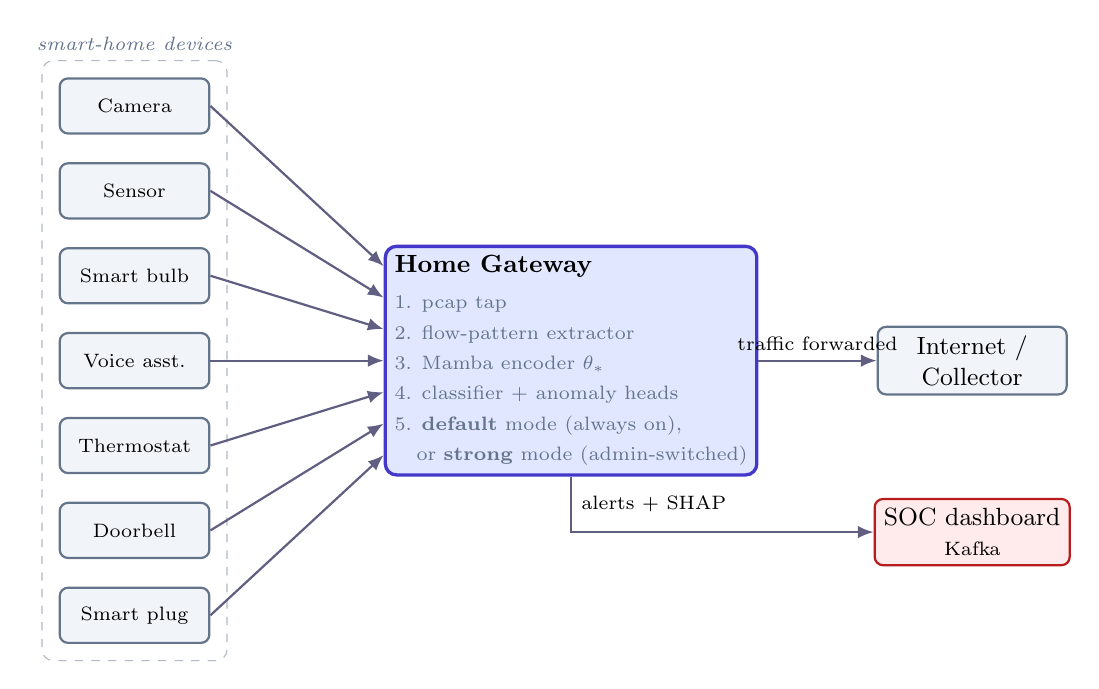
\begin{tikzpicture}[node distance=0.35cm and 1.2cm]

  % Devices around the gateway
  \node[iot] (cam)   {Camera};
  \node[iot, below=of cam]   (sen) {Sensor};
  \node[iot, below=of sen]   (bulb){Smart bulb};
  \node[iot, below=of bulb]  (va)  {Voice asst.};
  \node[iot, below=of va]    (thr) {Thermostat};
  \node[iot, below=of thr]   (door){Doorbell};
  \node[iot, below=of door]  (plug){Smart plug};

  \node[draw=mute!50, dashed, rounded corners, fit=(cam)(plug), inner sep=6pt,
        label={[font=\scriptsize\itshape, mute]above:smart-home devices}] (grp) {};

  % Gateway
  \node[hub, right=2.2cm of va] (gw)
       {\textbf{Home Gateway} \\[2pt]
        \scriptsize \color{mute} 1. pcap tap \\
        \scriptsize \color{mute} 2. flow-pattern extractor \\
        \scriptsize \color{mute} 3. Mamba encoder $\theta_*$ \\
        \scriptsize \color{mute} 4. classifier + anomaly heads \\
        \scriptsize \color{mute} 5. \textbf{default} mode (always on), \\
        \scriptsize \color{mute} \quad or \textbf{strong} mode (admin-switched)};

  % Downstream
  \node[data, right=1.5cm of gw, minimum width=2.4cm] (cc)
       {Internet / \\ Collector};
  \node[signal, below=1.3cm of cc, minimum width=2.4cm] (soc) {SOC dashboard \\ \scriptsize Kafka};

  % Arrows in
  \draw[ar] (cam.east)  -- ([yshift=1.2cm]gw.west);
  \draw[ar] (sen.east)  -- ([yshift=0.8cm]gw.west);
  \draw[ar] (bulb.east) -- ([yshift=0.4cm]gw.west);
  \draw[ar] (va.east)   -- (gw.west);
  \draw[ar] (thr.east)  -- ([yshift=-0.4cm]gw.west);
  \draw[ar] (door.east) -- ([yshift=-0.8cm]gw.west);
  \draw[ar] (plug.east) -- ([yshift=-1.2cm]gw.west);

  \draw[ar] (gw.east) -- node[above, font=\scriptsize]{traffic forwarded} (cc.west);
  \draw[ar] (gw.south) |- node[pos=0.25, right, font=\scriptsize]{alerts + SHAP} (soc.west);

\end{tikzpicture}
\caption*{\small\textit{Figure 1 --- The detector lives inside the home gateway. Device traffic continues to the internet unchanged; alerts and SHAP attributions are sent out-of-band to a SOC dashboard.}}
\end{figure}

% =======================================================================
\section{The approach in one diagram}

Conventional IoT IDS collapses each flow into a vector of $\sim$80 summary statistics (mean packet size, IAT standard deviation, flag counts, $\ldots$) before showing it to the model. This is convenient but \emph{permutation-invariant} --- you can shuffle the packets and the statistics don't change --- which destroys the temporal structure that attack signatures live in.

\begin{tcolorbox}[idea]
\textbf{Keep the order.} A flow is the first $K\!\approx\!32$ packets of the connection, kept as an ordered sequence $\mathbf{x} = (p_1, \ldots, p_K)$. Each $p_t$ is a small per-packet feature vector --- size, direction, inter-arrival time, TCP flags, header fields. A sequence model (Mamba) can then learn what a normal sequence looks like, and what a malicious one looks like.
\end{tcolorbox}

% ---- Figure 2: Representation contrast --------------------------------
\begin{figure}[H]
\centering
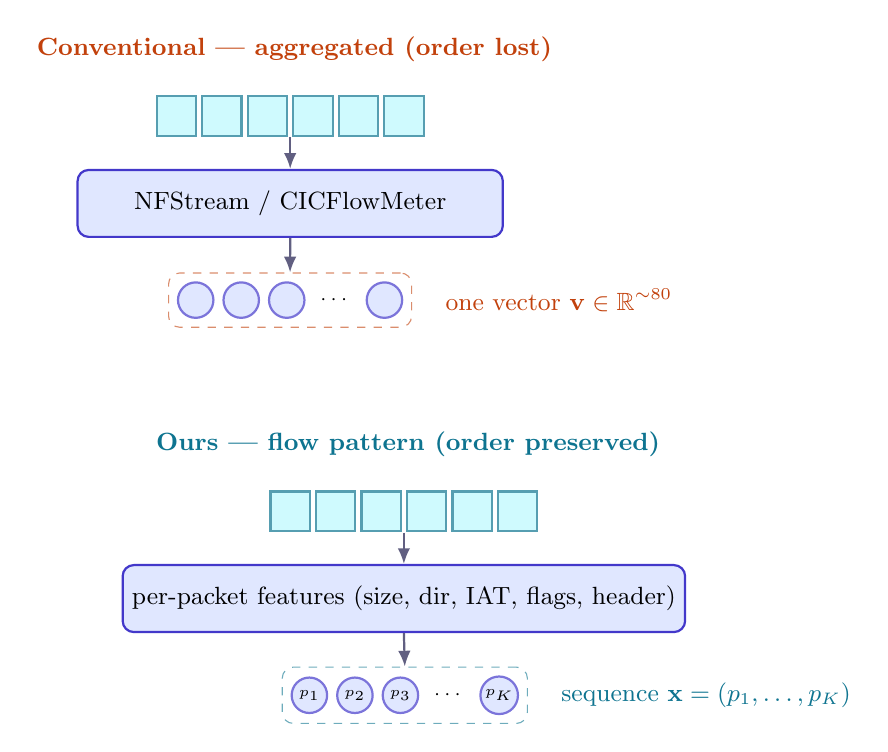
\begin{tikzpicture}[node distance=0.4cm and 0.9cm]

  % TOP row (conventional)
  \node[font=\bfseries\small, color=accent] (lhd) {Conventional --- aggregated (order lost)};

  \node[pkt, below=0.3cm of lhd, xshift=-1.5cm] (lp1) {};
  \node[pkt, right=0.05cm of lp1] (lp2) {};
  \node[pkt, right=0.05cm of lp2] (lp3) {};
  \node[pkt, right=0.05cm of lp3] (lp4) {};
  \node[pkt, right=0.05cm of lp4] (lp5) {};
  \node[pkt, right=0.05cm of lp5] (lp6) {};
  \node[fit=(lp1)(lp6), inner sep=0pt] (lpkts) {};

  \node[block, below=0.4cm of lpkts, minimum width=5.4cm] (lagg)
       {\small NFStream / CICFlowMeter};

  \node[bead, below=0.55cm of lagg, xshift=-1.2cm] (lf1) {};
  \node[bead, right=0.1cm of lf1] (lf2) {};
  \node[bead, right=0.1cm of lf2] (lf3) {};
  \node[right=0.06cm of lf3, font=\scriptsize] (ldots) {$\cdots$};
  \node[bead, right=0.06cm of ldots] (lf4) {};
  \node[draw=accent!60, dashed, rounded corners, fit=(lf1)(lf4), inner sep=3pt] (lvec) {};
  \node[right=0.3cm of lvec, font=\small, color=accent] {one vector $\mathbf{v}\in\mathbb{R}^{\sim 80}$};

  \draw[ar] (lpkts.south) -- (lagg.north);
  \draw[ar] (lagg.south) -- (lvec.north);

  % BOTTOM row (ours)
  \node[font=\bfseries\small, color=secondary, below=1.2cm of lvec, xshift=1.5cm] (rhd)
       {Ours --- flow pattern (order preserved)};

  \node[pkt, below=0.3cm of rhd, xshift=-1.5cm] (rp1) {};
  \node[pkt, right=0.05cm of rp1] (rp2) {};
  \node[pkt, right=0.05cm of rp2] (rp3) {};
  \node[pkt, right=0.05cm of rp3] (rp4) {};
  \node[pkt, right=0.05cm of rp4] (rp5) {};
  \node[pkt, right=0.05cm of rp5] (rp6) {};
  \node[fit=(rp1)(rp6), inner sep=0pt] (rpkts) {};

  \node[block, below=0.4cm of rpkts, minimum width=5.4cm] (ragg)
       {\small per-packet features (size, dir, IAT, flags, header)};

  \node[bead, below=0.55cm of ragg, xshift=-1.2cm] (rf1) {$p_1$};
  \node[bead, right=0.1cm of rf1] (rf2) {$p_2$};
  \node[bead, right=0.1cm of rf2] (rf3) {$p_3$};
  \node[right=0.06cm of rf3, font=\scriptsize] (rdots) {$\cdots$};
  \node[bead, right=0.06cm of rdots] (rf4) {$p_K$};
  \node[draw=secondary!60, dashed, rounded corners, fit=(rf1)(rf4), inner sep=3pt] (rvec) {};
  \node[right=0.3cm of rvec, font=\small, color=secondary] {sequence $\mathbf{x}=(p_1,\ldots,p_K)$};

  \draw[ar] (rpkts.south) -- (ragg.north);
  \draw[ar] (ragg.south) -- (rvec.north);

\end{tikzpicture}
\caption*{\small\textit{Figure 2 --- Two ways to feed a flow to a model. Aggregation collapses everything into one vector and drops ordering; the flow-pattern keeps the packets in order so a sequence model can use the temporal structure.}}
\end{figure}

% =======================================================================
\section{The architecture}

A single \textbf{Mamba encoder} processes the sequence $\mathbf{x}$ and produces a fixed-size embedding $\mathbf{z}$. Two heads then read $\mathbf{z}$, in parallel, for two purposes:

\begin{itemize}[leftmargin=*, itemsep=2pt]
  \item \textbf{Classifier head} --- a small MLP $\to$ softmax over the 7 known attack categories from CICIoT2023. Trained with focal loss to handle the heavy class imbalance.
  \item \textbf{Anomaly head} --- a one-class deep SVDD scorer, trained \emph{only on benign embeddings}. It does not know about any specific attack; it just measures distance from "normal."
\end{itemize}

\begin{tcolorbox}[idea]
\textbf{The anomaly head doesn't read $\mathbf{z}$ directly.} It reads a \textbf{projected} embedding $\mathbf{z}_\text{ano} = g_\phi(\mathbf{z})$ produced by a small learnable MLP (e.g.\ $\mathbb{R}^{128} \to \mathbb{R}^{32}$). One-class scorers like deep SVDD suffer from the curse of dimensionality --- in high dimensions, distances concentrate and lose discriminative power. Projecting down to a smaller anomaly space sharpens the score. The projection is trained jointly with the SVDD objective.
\end{tcolorbox}

\subsection{Why Mamba and not a transformer}
The reference architecture for pre-trained encrypted-traffic detectors is ET-BERT, a BERT-base-scale ($\sim$110M parameter) transformer. It works but doesn't fit on a Raspberry Pi. NetMamba (2024) showed that a Mamba state-space model achieves ET-BERT-class accuracy at substantially lower parameter and latency cost --- because Mamba runs in linear time in sequence length and has much lower per-token overhead than attention. We adopt that design.

\subsection{Why a shared encoder}
Pre-training is the expensive part. Sharing the encoder between both heads means we pay it once. It also gives the anomaly head a representation of "normal" that has been learned from a large benign corpus --- exactly what an anomaly scorer needs.

% =======================================================================
\section{Two operating modes --- default and strong}

The gateway can run in one of two configurations. The choice is an \textbf{operator-level setting} flipped by the admin, not a per-flow decision. One mode runs continuously by default; the other is switched on when the situation calls for it.

\begin{itemize}[leftmargin=*, itemsep=2pt]
  \item \textbf{Default mode --- low power, always on.} Smaller Mamba configuration, smaller $K$ (e.g., $K=8$), \emph{only the anomaly head} active, no SHAP. This is the baseline operating point: detection is on, the compute cost is small enough for continuous use on Raspberry-Pi-class hardware, and the system catches both known and novel attacks via the anomaly score alone.
  \item \textbf{Strong mode --- admin-switched, full pipeline.} Full Mamba configuration, $K=32$, \emph{both} classifier and anomaly heads (the latter via the projection MLP), plus SHAP attribution on every alert. Activated by the admin when needed --- elevated threat level, active incident investigation, high-value time window, or simply when the operator wants the maximum detection fidelity.
\end{itemize}

Switching is a configuration change applied to the gateway, not a per-flow decision and not an escalation. The same model artifacts --- encoder $\theta_*$, classifier head, projection, anomaly head --- are used in both modes; what differs is which components are engaged and at what size. Both modes produce alerts that go to the SOC. Strong mode additionally produces per-packet SHAP attributions for every alert.

% ---- Figure 3: Two-mode (admin-switched) inference --------------------
\begin{figure}[H]
\centering
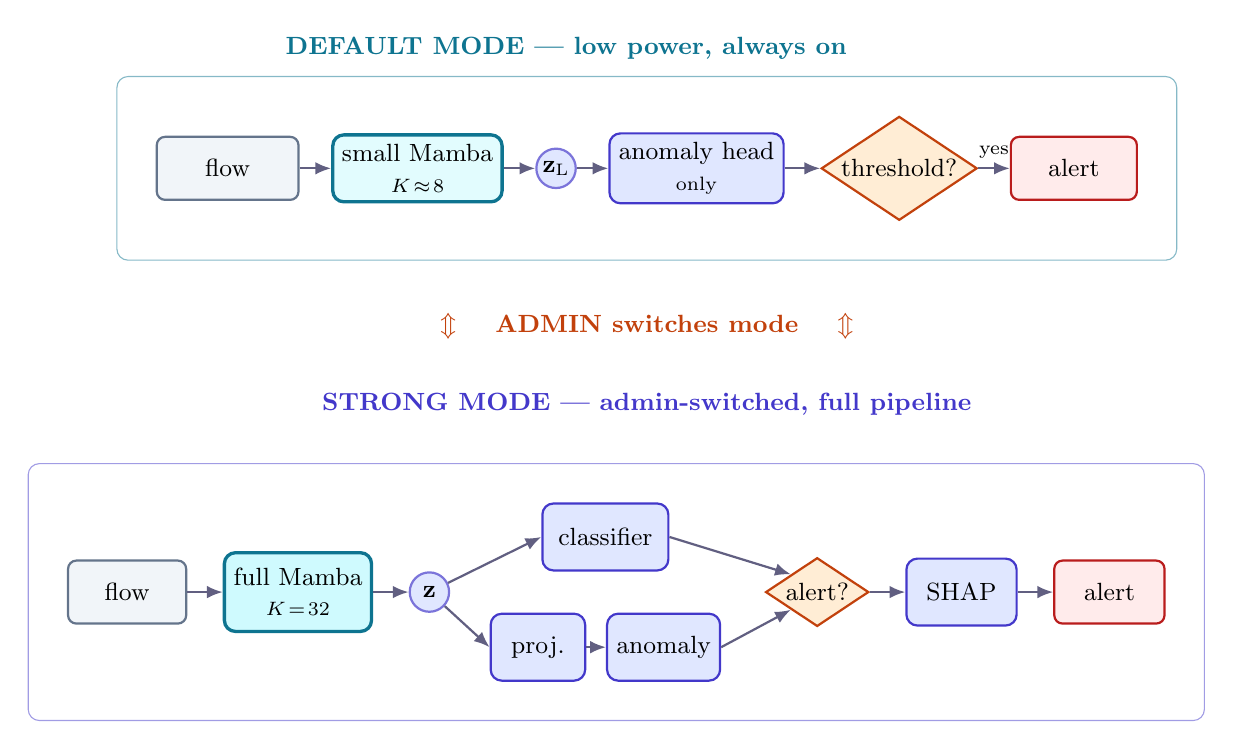
\begin{tikzpicture}[node distance=0.5cm and 0.55cm]

  % ----- DEFAULT MODE (top) -----
  \node[font=\bfseries\small\color{secondary}] (defhd) {DEFAULT MODE --- low power, always on};

  \node[data, below=0.85cm of defhd, xshift=-4.3cm, minimum width=1.8cm] (din) {flow};
  \node[brain, right=0.4cm of din, minimum width=2.0cm, minimum height=0.85cm, fill=secondarylight!60] (dmamba)
       {small Mamba \\ \scriptsize $K\!\approx\!8$};
  \node[bead, right=0.4cm of dmamba, minimum size=0.5cm, font=\small] (dz) {$\mathbf{z}_\text{L}$};
  \node[block, right=0.4cm of dz, minimum width=2.0cm] (dano) {anomaly head \\ \scriptsize only};
  \node[decision, right=0.45cm of dano] (dfuse) {threshold?};
  \node[signal, right=0.4cm of dfuse, minimum width=1.6cm] (dout) {alert};

  \draw[ar] (din) -- (dmamba);
  \draw[ar] (dmamba) -- (dz);
  \draw[ar] (dz) -- (dano);
  \draw[ar] (dano) -- (dfuse);
  \draw[ar] (dfuse) -- node[above, font=\scriptsize]{yes} (dout);

  \node[draw=secondary!50, rounded corners, fit=(din)(dout)(dmamba)(dano)(dfuse), inner sep=14pt] (sdef) {};

  % ----- Admin switch (middle) -----
  \node[below=0.55cm of sdef, font=\bfseries\small\color{accent}] (sw)
       {$\Updownarrow$ \quad ADMIN switches mode \quad $\Updownarrow$};

  % ----- STRONG MODE (bottom) -----
  \node[font=\bfseries\small\color{primary}, below=0.45cm of sw] (strhd)
       {STRONG MODE --- admin-switched, full pipeline};

  \node[data, below=1.7cm of strhd, xshift=-6.6cm, minimum width=1.5cm] (sin) {flow};
  \node[brain, right=0.45cm of sin, minimum width=1.8cm, minimum height=1.0cm] (smamba)
       {full Mamba \\ \scriptsize $K\!=\!32$};
  \node[bead, right=0.45cm of smamba, minimum size=0.5cm, font=\small] (sz) {$\mathbf{z}$};
  \node[block, right=0.5cm of sz, yshift=-0.7cm, minimum width=1.2cm] (sproj)
       {proj.};
  \node[block, right=0.25cm of sproj, minimum width=1.4cm] (sano) {anomaly};
  \coordinate (smid) at ($(sproj.west)!0.5!(sano.east)$);
  \node[block, minimum width=1.6cm] (scls) at ([yshift=1.4cm]smid) {classifier};
  \node[decision, right=0.55cm of sano, yshift=0.7cm] (sfuse) {alert?};
  \node[block, right=0.45cm of sfuse, minimum width=1.4cm] (sshap) {SHAP};
  \node[signal, right=0.45cm of sshap, minimum width=1.4cm] (sout) {alert};

  \draw[ar] (sin) -- (smamba);
  \draw[ar] (smamba) -- (sz);
  \draw[ar] (sz) -- (scls.west);
  \draw[ar] (sz) -- (sproj.west);
  \draw[ar] (sproj) -- (sano);
  \draw[ar] (scls.east) -- (sfuse.north west);
  \draw[ar] (sano.east) -- (sfuse.south west);
  \draw[ar] (sfuse) -- (sshap);
  \draw[ar] (sshap) -- (sout);

  \node[draw=primary!50, rounded corners, fit=(sin)(sout)(scls)(sproj)(sano)(sfuse)(sshap), inner sep=14pt] (sstr) {};

\end{tikzpicture}
\caption*{\small\textit{Figure 3 --- The two operating modes. Default mode runs continuously and uses only the lightweight anomaly head on a small Mamba. Strong mode is switched on by the admin and engages the full pipeline: full Mamba, classifier head, projected anomaly head, and SHAP attributions. The admin chooses which mode is active; the gateway then operates entirely in that mode until the next switch.}}
\end{figure}

% =======================================================================
\section{Training --- three stages, then a loop}

The detector is built in three stages. Each stage produces an artifact the next stage uses. The encoder is built first (without labels), then specialised with labels, then the anomaly head is added on top.

\subsection{Stage A --- Pre-train the encoder, no labels}
Take a large set of \textbf{benign} flows. Randomly mask ~15\% of packet positions in each sequence. Train the Mamba encoder to predict the masked packets from context. This is the SSL recipe pioneered by ET-BERT, applied to per-packet features. The output is an encoder $\theta_0$ that has learned what normal traffic looks like.

\subsection{Stage B --- Fine-tune with labels}
Attach a fresh classification head on top of $\theta_0$. Jointly fine-tune the encoder and the head on labelled CICIoT2023 attack data with focal loss. The output is the fine-tuned encoder $\theta_*$ and the trained classifier.

\subsection{Stage C --- Fit the anomaly head}
Freeze $\theta_*$. Push a held-out benign set through $\theta_*$ to get embeddings. Train the projection MLP and fit deep SVDD on the projected embeddings. Calibrate the threshold at the 99th percentile of benign scores (1\% FPR target).

\subsection{The loop --- absorbing new attack types}
When a previously unseen attack type appears in the wild, the system does \emph{not} need full retraining. The flow is:
\begin{enumerate}[leftmargin=*, itemsep=2pt]
  \item Anomaly head flags the novel attack on day zero (it just looks unlike normal).
  \item SOC labels a sample of the flagged flows as a new attack class.
  \item Extend the classifier softmax by one class and fine-tune \textbf{only the classifier head} on the new data, with a small replay buffer of old classes to prevent forgetting. The encoder $\theta_*$ stays frozen. Minutes, not days.
  \item Optionally recalibrate the anomaly threshold on a fresh benign set.
\end{enumerate}
Full encoder retraining is only triggered if the benign distribution itself shifts (new device types added to the network). This decoupling --- "what's normal" lives in the expensive encoder, "what's malicious" lives in the cheap heads --- is the operational payoff of the shared-encoder design.

% ---- Figure 4: Training stages + progressive loop ---------------------
\begin{figure}[H]
\centering
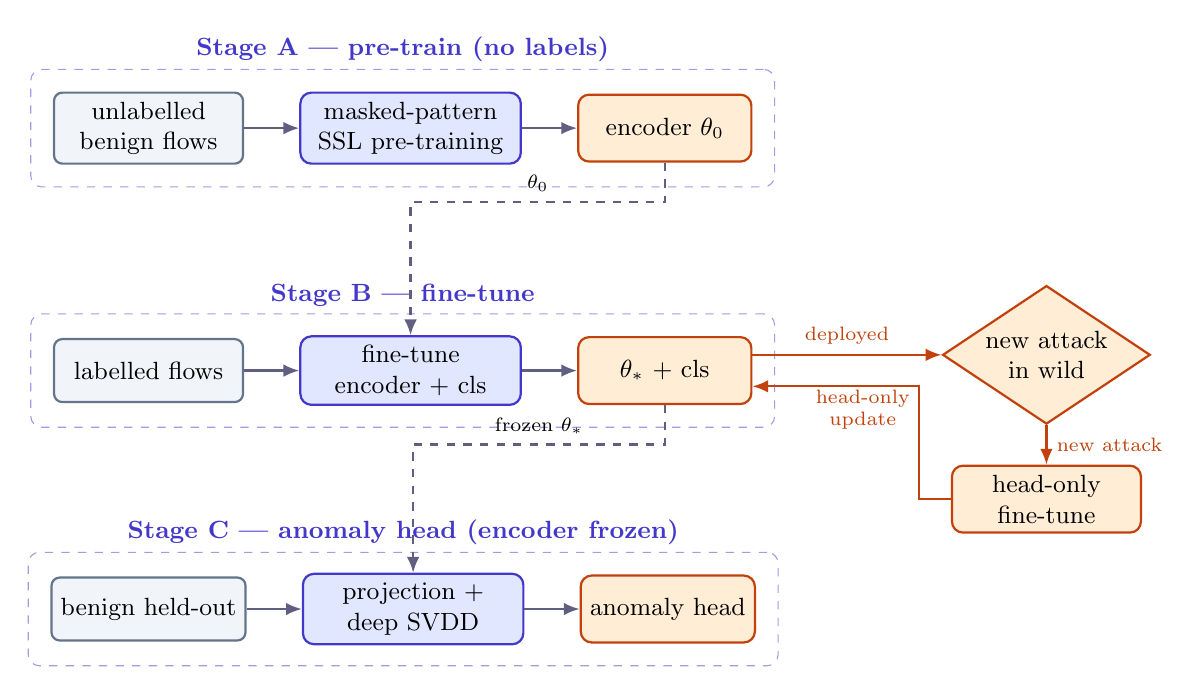
\begin{tikzpicture}[node distance=0.55cm and 0.7cm]

  % Stage A
  \node[data, minimum width=2.4cm] (a1) {unlabelled \\ benign flows};
  \node[block, right=of a1, minimum width=2.8cm] (a2)
       {masked-pattern \\ SSL pre-training};
  \node[art, right=of a2, minimum width=2.2cm] (a3) {encoder $\theta_0$};
  \node[draw=primary!50, dashed, rounded corners, fit=(a1)(a3), inner sep=8pt,
        label={[font=\small\bfseries\color{primary}, above=-1pt]:Stage A --- pre-train (no labels)}] (sA) {};
  \draw[ar] (a1) -- (a2);
  \draw[ar] (a2) -- (a3);

  % Stage B
  \node[data, minimum width=2.4cm, below=2.2cm of a1] (b1) {labelled flows};
  \node[block, right=of b1, minimum width=2.8cm] (b2)
       {fine-tune \\ encoder + cls};
  \node[art, right=of b2, minimum width=2.2cm] (b3) {$\theta_*$ + cls};
  \node[draw=primary!50, dashed, rounded corners, fit=(b1)(b3), inner sep=8pt,
        label={[font=\small\bfseries\color{primary}, above=-1pt]:Stage B --- fine-tune}] (sB) {};
  \draw[ar] (b1) -- (b2);
  \draw[ar] (b2) -- (b3);
  \draw[dar] (a3.south) -- ++(0,-0.5) -| node[pos=0.25, above, font=\scriptsize]{$\theta_0$} (b2.north);

  % Stage C
  \node[data, minimum width=2.4cm, below=2.2cm of b1] (c1) {benign held-out};
  \node[block, right=of c1, minimum width=2.8cm] (c2)
       {projection + \\ deep SVDD};
  \node[art, right=of c2, minimum width=2.2cm] (c3) {anomaly head};
  \node[draw=primary!50, dashed, rounded corners, fit=(c1)(c3), inner sep=8pt,
        label={[font=\small\bfseries\color{primary}, above=-1pt]:Stage C --- anomaly head (encoder frozen)}] (sC) {};
  \draw[ar] (c1) -- (c2);
  \draw[ar] (c2) -- (c3);
  \draw[dar] (b3.south) -- ++(0,-0.5) -| node[pos=0.25, above, font=\scriptsize]{frozen $\theta_*$} (c2.north);

  % Progressive learning loop (to the right of everything)
  \node[decision, right=2.4cm of b3, yshift=0.2cm, fill=accentlight] (newatk)
       {new attack \\ in wild};
  \node[block, below=0.5cm of newatk, minimum width=2.4cm, fill=accentlight, draw=accent] (heads)
       {head-only \\ fine-tune};

  \draw[ar, draw=accent, line width=0.8pt] ([yshift=0.2cm]b3.east) -- node[above, font=\scriptsize\color{accent}]{deployed} (newatk.west);
  \draw[ar, draw=accent, line width=0.8pt] (newatk) -- node[right, font=\scriptsize\color{accent}]{new attack} (heads);
  % Return arrow: short hop LEFT from heads, vertical UP outside Stage B rectangle, horizontal back into b3.east (offset DOWN so it doesn't merge with the outgoing 'deployed' arrow)
  \draw[ar, draw=accent, line width=0.8pt]
    (heads.west) -- ++(-0.4, 0)
    |- ([yshift=-0.2cm]b3.east);

  % Label placed independently in the empty space just below b3, right of the Stage B rectangle
  \node[font=\scriptsize\color{accent}, align=center]
    at ([xshift=1.4cm, yshift=-0.5cm]b3.east)
    {head-only \\ update};

\end{tikzpicture}
\caption*{\small\textit{Figure 4 --- The three training stages produce the deployed detector. The amber loop on the right is the progressive-learning path: when a new attack arrives, only the lightweight classifier head is re-trained --- the expensive encoder stays put.}}
\end{figure}

% =======================================================================
\section{Evaluation}

\subsection{Datasets}
\textbf{CICIoT2023} (primary). \textbf{TON\_IoT} for cross-dataset generalisation --- trained model evaluated on a dataset it has never seen. \textbf{IoT-23} for a real-world malware check (Mirai, Torii, Okiru, Gafgyt).

\subsection{Baselines --- and what each one is for}
\begin{itemize}[leftmargin=*, itemsep=2pt]
  \item \textbf{ET-BERT} --- the published-SOTA upper bound. Tells us how much accuracy we leave on the table by going to Mamba.
  \item \textbf{CNN-BiLSTM on aggregated statistics} --- the representation control. Isolates the gain from the flow-pattern input.
  \item \textbf{XGBoost on aggregated statistics} --- the \emph{classical-floor challenge}. In IDS literature, gradient-boosted trees on hand-crafted features are routinely competitive with deep models. We keep XGBoost as an explicit baseline to answer the ``do we need deep learning at all?'' question. The deep detector only earns its complexity if it beats XGBoost on the metrics XGBoost cannot target: \textbf{zero-day detection} (XGBoost is supervised-only), \textbf{cross-dataset transfer} (the pre-trained encoder is the bet), and \textbf{adversarial robustness}. If XGBoost matches us in-distribution, we report that as a finding.
  \item \textbf{Isolation Forest} --- the classical unsupervised floor against which the anomaly head is judged.
\end{itemize}

\subsection{Metrics}
Per-class precision / recall / F1. PR-AUC (the honest metric under heavy class imbalance). Inference latency p50 / p95 / p99 per flow. Model size in MB after int8 quantisation.

\subsection{Adversarial study}
Fast Gradient Sign Method (FGSM) on the per-packet sequence, perturbations clipped to valid feature ranges. Detection rate vs.\ perturbation magnitude $\varepsilon$, plotted for both heads. Secondary check: do SHAP attribution patterns on adversarial inputs differ from those on clean inputs? (They tend to --- a useful fallback signal.)

\subsection{Zero-day proxy}
Leave-one-class-out: hide an attack class from the supervised head during Stage B, then measure how well the anomaly head detects it at test time. Repeat per class. This is our concrete answer to "how do you evaluate something you haven't trained on."

% =======================================================================
\section{Plan, deliverables, risks}

\subsection{Twelve-week plan}
Weeks 1--2 setup and dataset validation; week 3 flow-pattern extractor and classical baselines; weeks 4--5 Stage A pre-training; week 6 Stage B fine-tuning and bring up CNN-BiLSTM + ET-BERT comparison; week 7 Stage C anomaly head and leave-one-class-out; week 8 TON\_IoT + IoT-23 evaluation; week 9 SHAP integration; week 10 FGSM adversarial study; week 11 int8 quantisation and gateway latency benchmark; week 12 stretch goal (if time), final report, presentation.

\subsection{Deliverables}
Reproducible code repository covering the full pipeline. Pre-trained Mamba encoder checkpoint $\theta_*$ released alongside the report. Benchmark table covering Mamba vs.\ ET-BERT vs.\ CNN-BiLSTM vs.\ XGBoost vs.\ Isolation Forest across CICIoT2023, TON\_IoT, IoT-23. FGSM degradation curves. Latency / memory profile on gateway hardware. Written report.

\subsection{Risks --- and what I do about them}
\begin{tcolorbox}[warnbox]
\begin{itemize}[leftmargin=*, itemsep=1pt, topsep=0pt]
  \item \textbf{Pre-training compute blows budget.} Warm-start from a public Mamba checkpoint and adapt on benign IoT traffic rather than train from scratch.
  \item \textbf{Class imbalance hides minority-class failure.} Focal loss + always report per-class metrics.
  \item \textbf{Cross-dataset accuracy drop.} Measure honestly; this is the standard caveat in IDS literature, not a failure mode to hide.
  \item \textbf{Edge memory overrun.} Int8 quantise. Fall back to a smaller Mamba configuration. Reduce $K$ as a last resort.
  \item \textbf{Byte-level adversarial sensitivity.} The FGSM study quantifies it explicitly. SHAP fingerprint as a secondary defence.
\end{itemize}
\end{tcolorbox}

\subsection{Stretch goals}
\begin{itemize}[leftmargin=*, itemsep=1pt]
  \item Swap Mamba $\to$ Mamba-2 (Structured State Space Duality) if latency headroom allows.
  \item Add an E-GraphSAGE branch over a per-window device-communication graph.
  \item Federated pre-training across multiple homes / sites.
\end{itemize}

% =======================================================================
\section{Key references}
\footnotesize
\begin{itemize}[leftmargin=*, itemsep=1pt]
  \item \textbf{NetMamba}, Wang et al.\ 2024 --- \href{https://arxiv.org/abs/2405.11449}{arxiv.org/abs/2405.11449}
  \item \textbf{ET-BERT}, Lin et al.\ WWW 2022 --- \href{https://arxiv.org/abs/2202.06335}{arxiv.org/abs/2202.06335}
  \item \textbf{Mamba}, Gu \& Dao 2023 --- \href{https://arxiv.org/abs/2312.00752}{arxiv.org/abs/2312.00752}
  \item \textbf{Mamba-2 / SSD}, Dao \& Gu 2024 --- \href{https://arxiv.org/abs/2405.21060}{arxiv.org/abs/2405.21060}
  \item \textbf{S4D}, Gu, Goel, R\'e 2022 --- \href{https://arxiv.org/abs/2206.11893}{arxiv.org/abs/2206.11893}
  \item \textbf{CICIoT2023}, Neto et al.\ 2023 --- \href{https://www.mdpi.com/1424-8220/23/13/5941}{mdpi.com/1424-8220/23/13/5941}
  \item \textbf{Deep SVDD}, Ruff et al.\ ICML 2018 --- the one-class anomaly scorer
  \item \textbf{ET-SSL}, Nature Sci.\ Rep.\ 2025 --- contrastive SSL on encrypted traffic
  \item \textbf{E-GraphSAGE}, Lo et al. --- \href{https://arxiv.org/abs/2103.16329}{arxiv.org/abs/2103.16329}
\end{itemize}

\end{document}
